\chapter{Wyniki testów}
\label{ch:tests}

$TODO$
obszerne testy, porównanie metod przy tych samych warunkach początkowych
do przeprowadzenia testów wykorzystano biblitekę jUnit, która co prawda służy do wykonywania testów jednostkowych sprawdzających poprawność pojedynczych komponentów aplikacji
metodyka przeprowadzenia testów
przeprowadzenie testów jest trudne i wymaga losowania środowisk i warunków i wyciągania statystyki, brak porównania do absolutu, ale można porównać różne metody w tych samych wylosowanych mapach - te same warunki początkowe
jak whca* nie zadziała, nie wiadomo, czy w ogole nie ma rozwiazania
potential field - nawet nie warto testować, raczej jako ciekawostka, nie potrafi doprowadzić do celu nawet jednego robota, screen z minimum lokalnego - studni potencjału
ile wszystkich symulacji przeprowadzono
testy powodzenia (skuteczności i wydajnosci) i testy poprawności (różnica)
histogram liczby kroków potrzebnych do rozwiązania
WHCA* z różnym parametrem okna czasowego

\section{Środowiska testowe}
Testy zostały przeprowadzone na 4 typach losowych środowisk:
\begin{itemize}
	\item mapa rozmiaru $15 \times 15$ z wygenerowanym labiryntem, 5 robotów na mapie (por. rys. \ref{fig:test-env-15-15-5}),
	\item mapa rozmiaru $15 \times 15$ z wygenerowanym labiryntem, 10 robotów na mapie (por. rys. \ref{fig:test-env-15-15-10}),
	\item mapa rozmiaru $35 \times 35$ z wygenerowanym labiryntem, 5 robotów na mapie (por. rys. \ref{fig:test-env-35-35-5}),
	\item mapa rozmiaru $15 \times 15$ bez przeszkód, 40 robotów na mapie (por. rys. \ref{fig:test-env-15-15-empty-40}).
\end{itemize}
Dla każdego typu środowiska za każdym razem generowana jest nowa, losowa mapa. Również położenie początkowe i docelowe robotów jest lososwane. Zatem w każdej symulacji wykorzystywane jest inne środowisko, chyba, że porównywane są między sobą różne metody. Wtedy rekonstruowane są te same warunki początkowe, aby przeprowadzić symulację ponownnie z wykorzystaniem innej metody planowania.

Każdy z robotów otrzymuje losowe położenie początkowe. Jest to zawsze pole, na którym nie znajduje się przeszkoda, ani nie ma na nim innego robota.
Punkty docelowe także są losowane. Mogą to być pola, na których obecnie znajduje się jakiś robot, natomiast nie może to być punkt docelowy należący do innego robota, gdyż w przeciwnym wypadku uniemożliwiłoby to znalezienie rozwiązania, niezależnie od metody planowania.

\begin{figure}
	\centering
	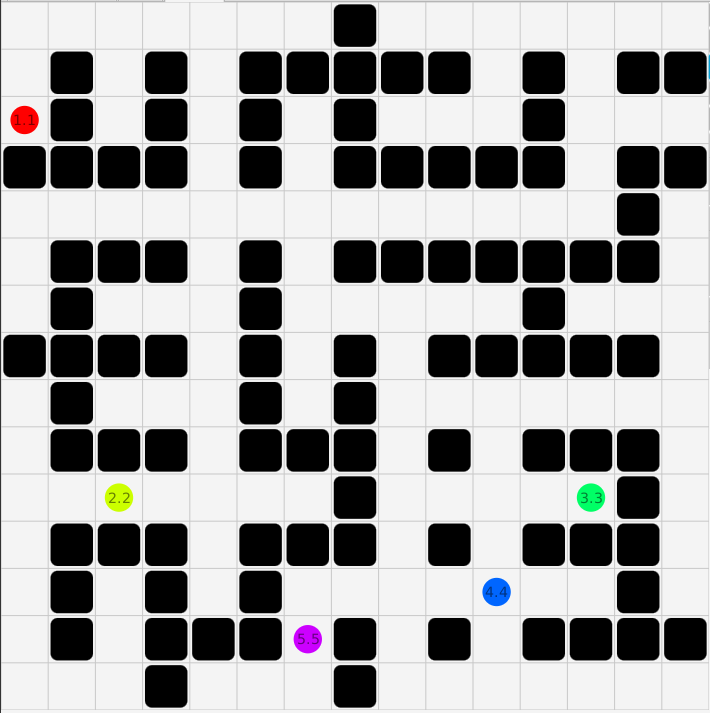
\includegraphics[width=0.6\columnwidth]{img/robopath/tests-15-15-5}
	\caption{Mapa $15 \times 15$ z wygenerowanym labiryntem, z 5 robotami w losowych położeniach}
	\label{fig:test-env-15-15-5}
\end{figure}

\begin{figure}
	\centering
	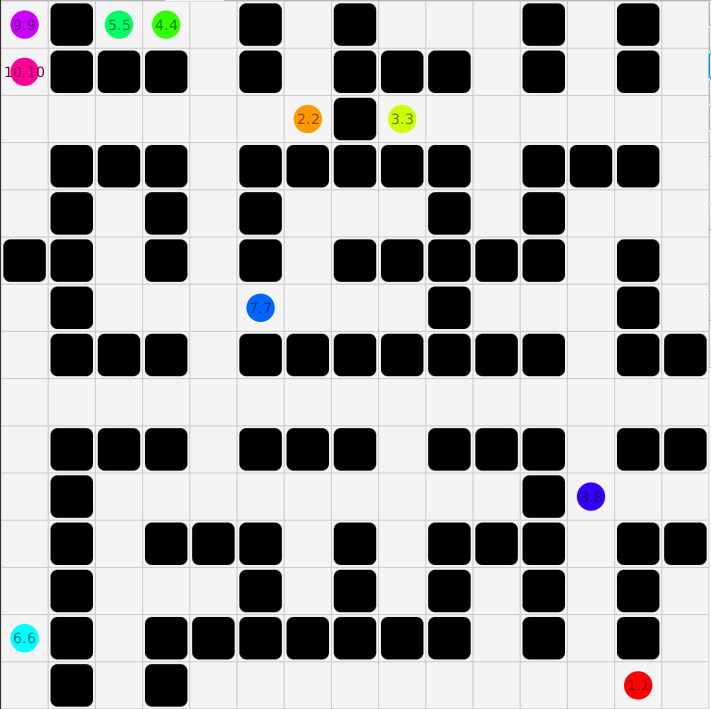
\includegraphics[width=0.6\columnwidth]{img/robopath/tests-15-15-10}
	\caption{Mapa $15 \times 15$ z wygenerowanym labiryntem, z 10 robotami w losowych położeniach}
	\label{fig:test-env-15-15-10}
\end{figure}

\begin{figure}
	\centering
	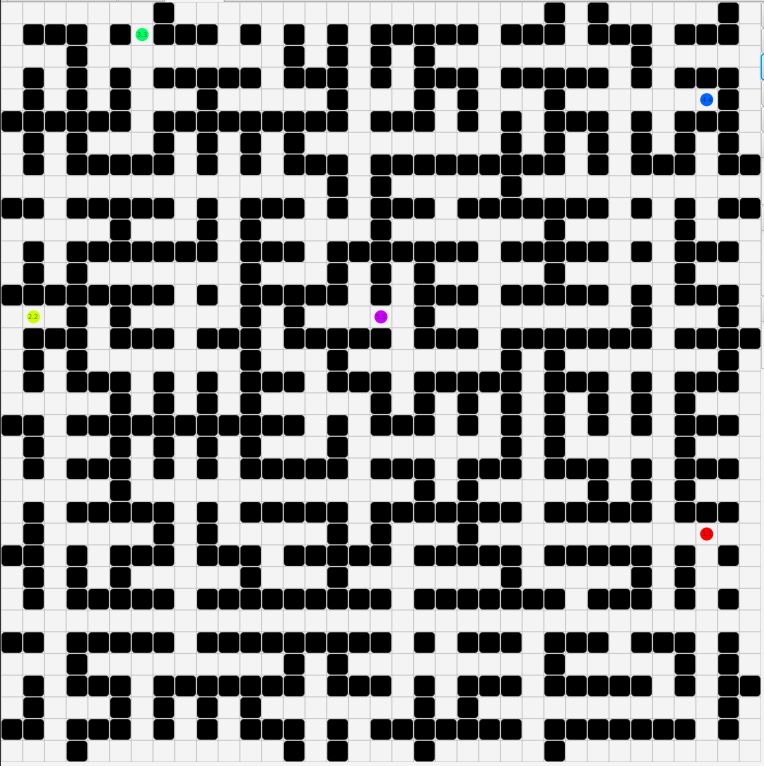
\includegraphics[width=0.6\columnwidth]{img/robopath/tests-35-35-5}
	\caption{Mapa $35 \times 35$ z wygenerowanym labiryntem, z 5 robotami w losowych położeniach}
	\label{fig:test-env-35-35-5}
\end{figure}

\begin{figure}
	\centering
	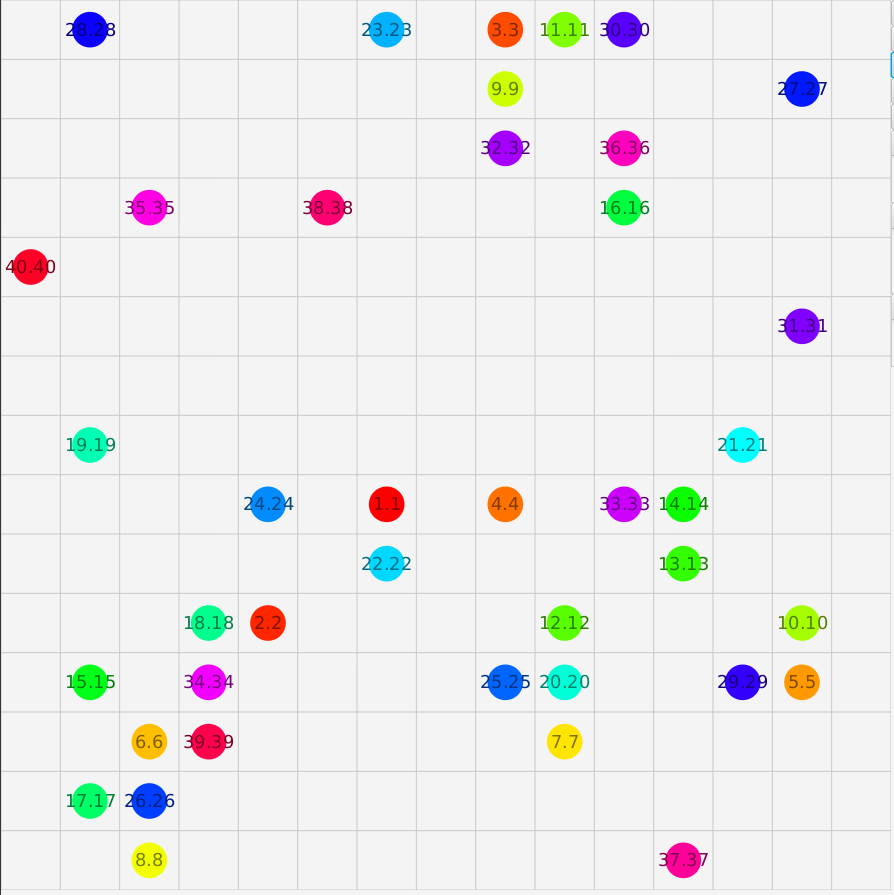
\includegraphics[width=0.6\columnwidth]{img/robopath/tests-15-15-empty-40}
	\caption{Mapa $15 \times 15$ bez przeszkód, z 40 robotami w losowych położeniach}
	\label{fig:test-env-15-15-empty-40}
\end{figure}

Przetestowane metody:
\begin{itemize}
	\item algorytm A* bez rozwiązywania kolizji
	\item LRA*
	\item WHCA* bez dynamicznego przydzielania priotytetów
	\item WHCA* z dynamicznym przydziałem priorytetów
	\item WHCA* z dynamicznym przydziałem priorytetów oraz dynamicznym skalowaniem okna czasowego
\end{itemize}

Zmierzone wskaźniki:
\begin{itemize}
	\item fakt doprowadzenia wszystkich robotów do celów wzdłuż bezkolizyjnych tras, skuteczność = liczba udanych / wszystkich
	\item liczba potrzebnych kroków symulacji (czas wykonywania akcji w rzeczywistym środowisku)
	\item czas wykonywania planowania (wykonywania obliczeń dla wszystkich kroków symulacji)
\end{itemize}

\section{Wyniki testów}
\subsection{Częstotliwość występowania kolizji}
najpierw pokazujemy, że rozwiązywanie kolizji jest potrzebne na tego typu mapach - sam A* nie wystarcza

\section{Charakterystyczne przypadki}
$TODO$ screeny ciekawych przypadków

\begin{figure}
	\centering
	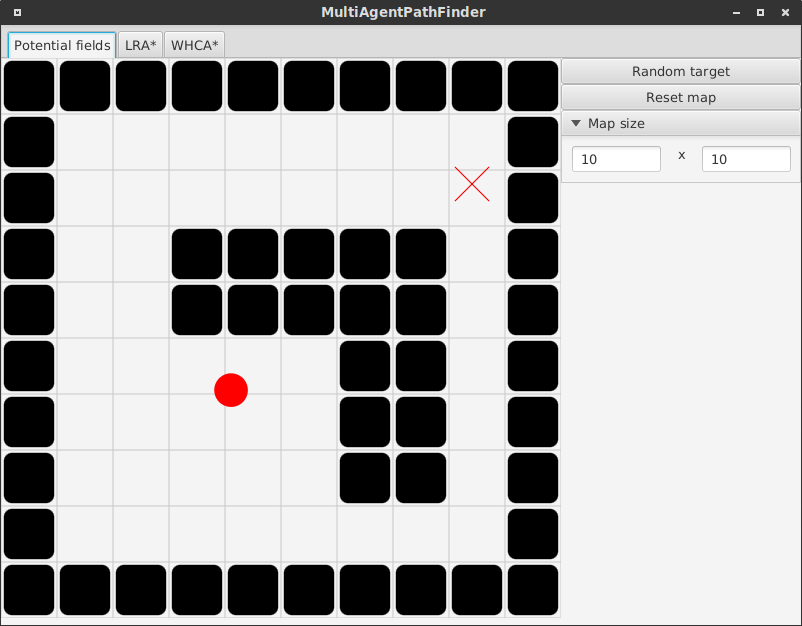
\includegraphics[width=0.8\columnwidth]{img/robopath/field-potential-hole}
	\caption{Robot uwięziony w studni potencjału. Zerowa siła wypadkowa nie pozwala mu dotrzeć do celu.}
	\label{fig:test-field-potential-hole}
\end{figure}

\begin{figure}
	\centering
	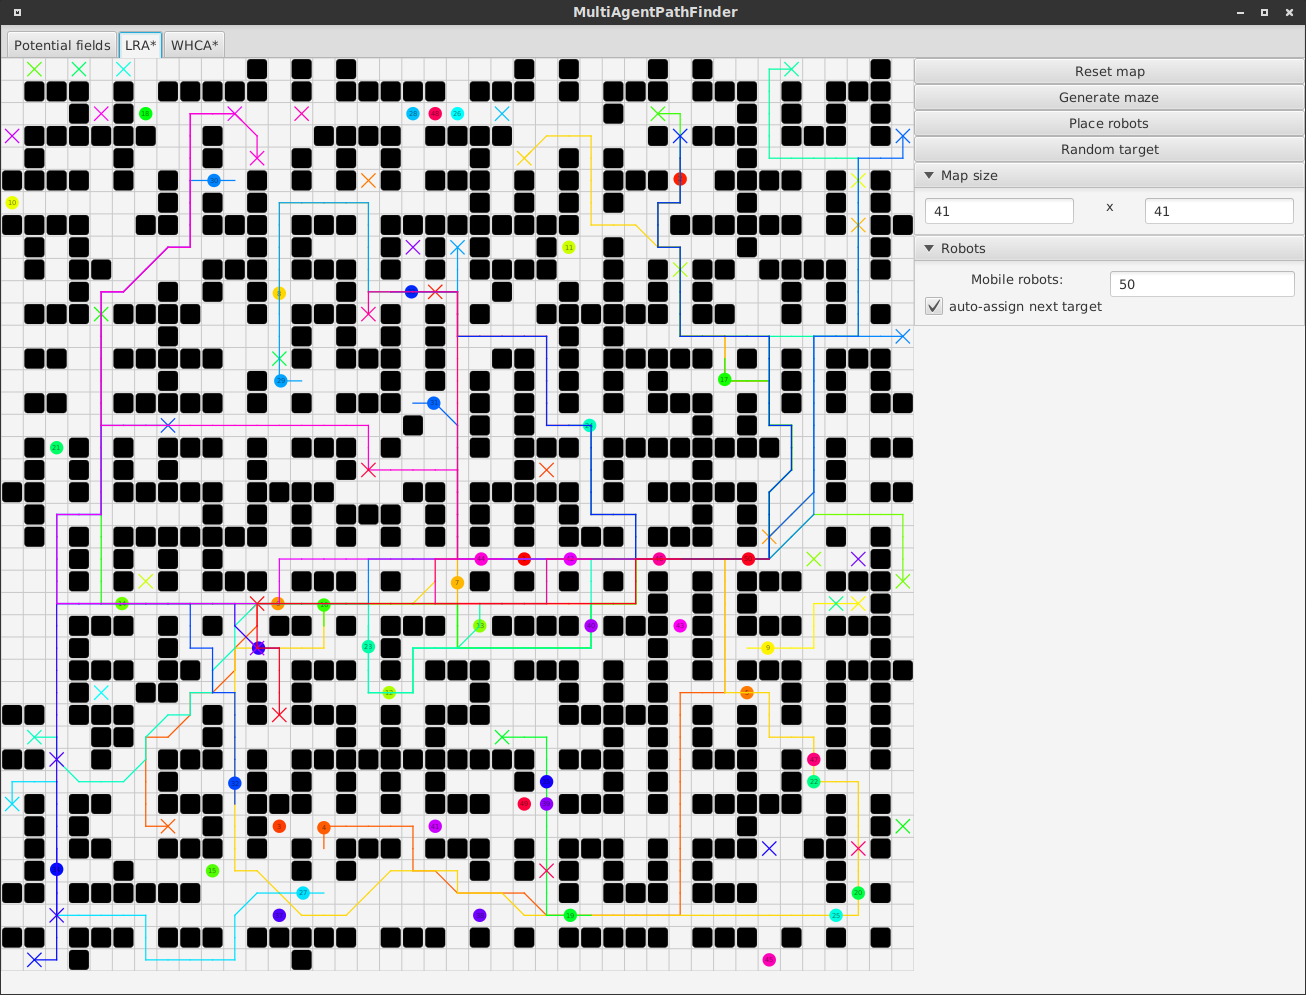
\includegraphics[width=0.8\columnwidth]{img/robopath/lra-bigmap}
	\caption{Metoda LRA*: duża mapa z dużą liczbą robotów}
	\label{fig:test-lra-bigmap}
\end{figure}

\begin{figure}
	\centering
	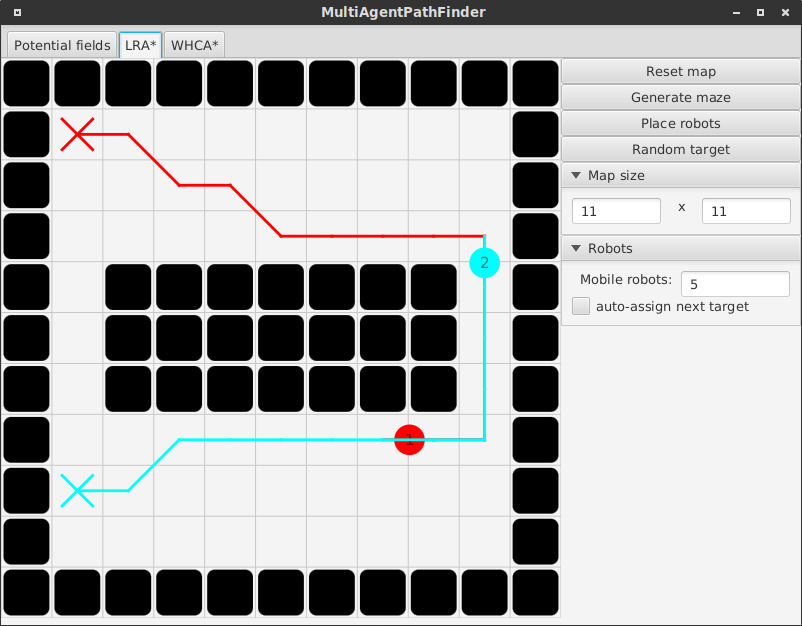
\includegraphics[width=0.8\columnwidth]{img/robopath/lra-cycle}
	\caption{Metoda LRA*: 2 roboty w cyklu akcji}
	\label{fig:test-lra-cycle}
\end{figure}

\begin{figure}
	\centering
	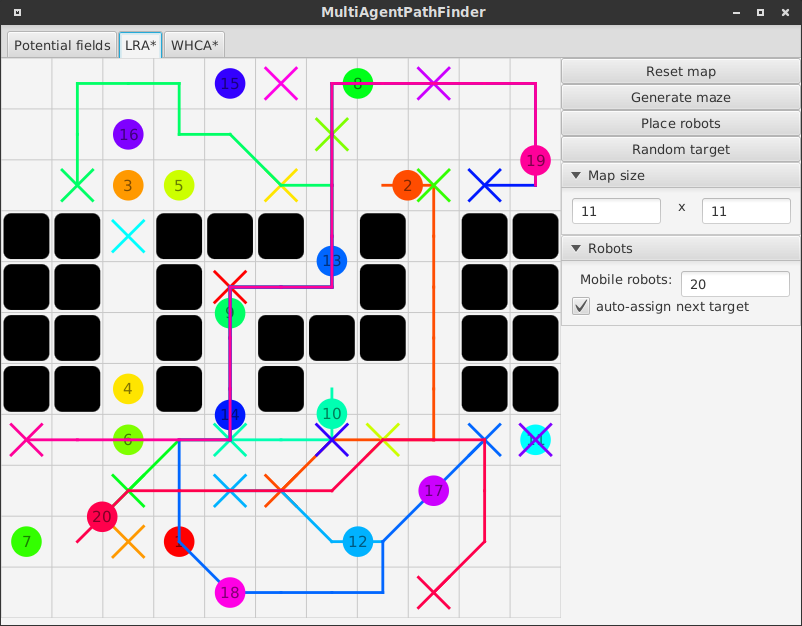
\includegraphics[width=0.8\columnwidth]{img/robopath/lra-lot-robots}
	\caption{Metoda LRA*: dużo robotów, mała mapa}
	\label{fig:test-lra-lot-robots}
\end{figure}

\begin{figure}
	\centering
	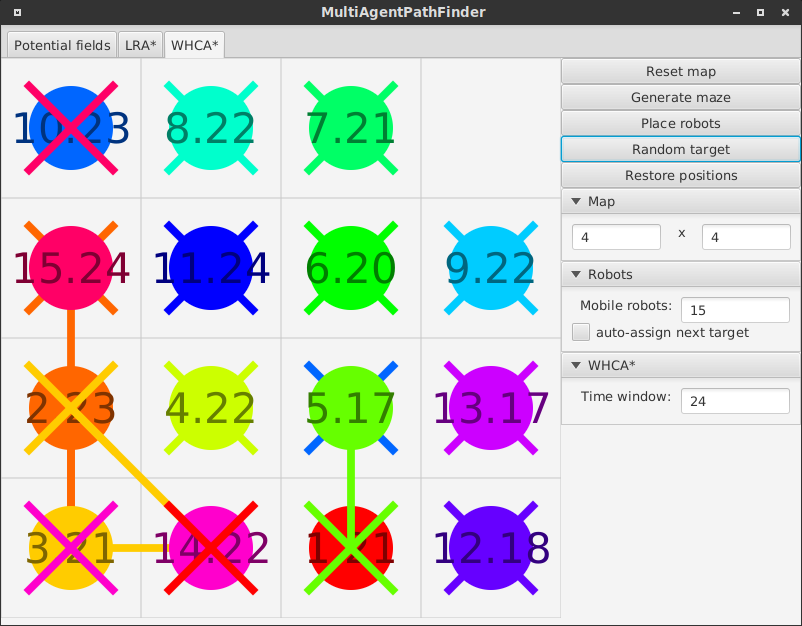
\includegraphics[width=0.8\columnwidth]{img/robopath/puzzle-15}
	\caption{Metoda WHCA*: puzzle 15}
	\label{fig:test-puzzle-15}
\end{figure}

puzzle 15
LRA: wyszło całkiem nieźle w przypadku, gdy do celu prowadzi wiele alternatywnych ścieżek i można ominąć wąskie gardło
testy ograniczać trzeba liczbą kroków symulacji, bo LRA może trwać wiecznie

\section{Porównanie wyników}
jak często zwykły A* to za mało - ile razy pojawia się chociaż jedna kolizja?
porównanie WHCA* przy różnych oknach czasowych
porównanie metod przydziału i zmiany priorytetów - jak zmienia się skuteczność  po wprowadzeniu zmiany priorytetów
porównanie LRA* z WHCA*
porównanie CA* z WHCA*
porównanie z potential fields
porównanie WHCA z promocją priorytetów (własną, autorską) i bez + z/bez rozszerzania okna czasowego

\section{Dyskusja wyników}
potwierdzenie oczekiwań (poprawności) - nigdy nie było tak, żeby LRA był lepszy

wolno działa WHCA* przy dużych mapach / oknach czasu / robotach. Dałoby się zoptymalizować (RRA)
autorski WHCA* działa dobrze nawet przy rozwiązywaniu dużych deadlocków, problem z puzzle 15

wada - nie moze się dwóch agentów "cofać". MOże tylko uciekać  z drogi ważniesjzemu